Let us define: \\ \\
$
    \begin{aligned}
        Size(O(1)) = \{ & \lang : \text{ There exists a circuit ensemble } C=\{C_n\}_{n \in \nat} \\
                        & \text{such that } \lang(C)=\lang \text{ and } |C_n|\in O(1\}
    \end{aligned}
$ \\ \\
We will present a non-regular $\lang$ such that $\lang \in Size(O(1))$.

We will use the language in question 3c: \\
$\lang=\{w : \exists n \in \nat \text{ s.t. } |w| = n^3\}$ \\
it was proven in 3c that the above language is not regular.

We can construct the following circuit ensemble $C=\{C_n\}_{n \in \nat}$ \\
such that $\lang(C)=\lang$ and $|C_n|\in O(1\}$:

if $n$ is a cube of an integer ($\sqrt[3]{n} \in \nat$), then the circuit, $C_n$, will return the constant 1, \\
otherwise (if $\sqrt[3]{n} \notin \nat$) the circuit, $C_n$, will return the constant 0.

Presenting the above as formula:
$
    C_n(x_1 ... x_n) =
    \begin{cases}
        1 , & \sqrt[3]{n} \in \nat    \\
        0 , & \sqrt[3]{n} \notin \nat \\
    \end{cases}
$

Presenting as a diagram: \\
\textcolor{red}
{
    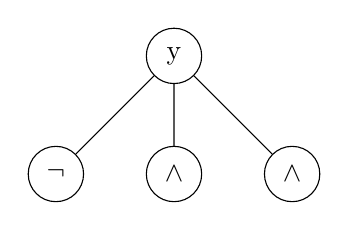
\begin{tikzpicture}[
            every node/.style = {minimum width = 2em, draw, circle},
        ]
        \node {y}
        child {node {$\neg$}}
        child {node {$\wedge$}}
        child {node {$\wedge$}};
    \end{tikzpicture}
}

Indeed, $w \in \lang$ iff then $C_{|w|}(w)=1$.
Therefore $\lang(C)=\lang$ and for each circuit in the ensemble $|C_n| = 0 \in O(1\}$ since there are no logic
gates in all the circuits in the ensemble.